\section{Resultados sobre métodos aleatorizados}

En esta sección nos dedicaremos a analizar qué propiedades verifican los métodos enunciados anteriormente. 
Principalmente nos interesarán los métodos que verifiquen \textit{monotonía de selección}, puesto que 
por construcción sabemos que todos los métodos verifican \textit{quota}, y también hemos visto que varios
de ellos verifican \textit{proporcionalidad ex-ante}.

\subsection{Método de Grimmett - \textit{Systematic rounding}}

Hemos visto que este método verifica \textit{proporcionalidad ex-ante}. 
Para mostrar que no verifica \textit{monotonía de selección}, tomaremos el contraejemplo propuesto en 
\cita{correa2024monotonerandomizedapportionment} en la isla ficticia de \textit{Apportia}. Se propone un escenario en el que se 
reparten 11 bancas entre 6 partidos pertenecientes a dos coaliciones políticas distintas: 3 de ellos de izquierda, 
los 3 restantes de derecha. Para ver que no se cumple \textit{monotonía de selección}, basta mostrar una forma de modificar los 
perfiles de votos, trasladando votos propios de la coalición de izquierda a la coalición de derecha, y viendo que a pesar 
de que la izquierda pierde votos, la probabilidad de que las 3 bancas sean asignadas a los partidos de dicha coalición aumenta.

\begin{table}[h!]
\centering
\begin{tabular}{l l r r r r r r}
\toprule
\textbf{Partido} & \textbf{Coalición} &
\multicolumn{3}{c}{\textbf{Elección anterior}} & \multicolumn{3}{c}{\textbf{Nueva elección}} \\
\cmidrule(lr){3-5}\cmidrule(lr){6-8}
 & & \textbf{Votos} & \textbf{Quota inf.} & \textbf{Resto} & \textbf{Votos} & \textbf{Quota inf.} & \textbf{Residuo} \\
\midrule
1 & izquierda  & 110 & 1 & 0.1 & 110 & 1 & 0.1 \\
2 & derecha    & 270 & 2 & 0.7 & \chgpos{+20} \ 290 & 2 & 0.9 \\
3 & izquierda  & 210 & 2 & 0.1 & 210 & 2 & 0.1 \\
4 & derecha    & 160 & 1 & 0.6 & \chgpos{+30} \ 190 & 1 & 0.9 \\
5 & izquierda  &  70 & 0 & 0.7 & \chgneg{-60} \ \ 10 & 0 & 0.1 \\
6 & derecha    & 280 & 2 & 0.8 & \chgpos{+10} \ 290 & 2 & 0.9 \\
\bottomrule
\end{tabular}
\caption{Compración de votos y restos entre elecciones. Extraído de \cita{correa2024monotonerandomizedapportionment}.}
\label{tab:comparacion-elecciones}
\end{table}

\FloatBarrier

\begin{figure}[h!]
    \centering
    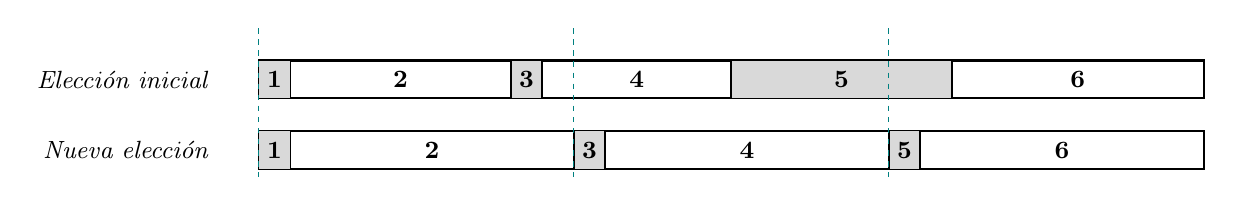
\begin{tikzpicture}[every node/.style={font=\small}]
    
    % parámetros
    \def\W{12}        % ancho total de la barra (cm)
    \def\nseats{6}    % número de casillas
    \def\w{\W/\nseats} % ancho por casilla
    
    % coordenadas de las dos barras (y)
    \def\yTop{1.6}
    \def\yBottom{0.0}
    \def\gap{0.9}     % separación vertical entre barras
    
    % colores
    \definecolor{dashcolor}{RGB}{0,128,128} % color de líneas punteadas
    \definecolor{shadeleft}{gray}{0.85}     % color para partidos "izquierda"
    
    % --- Barra superior: Previous election ---
    \begin{scope}
      \coordinate (left) at (0,0);
      % rectángulo marco
      \draw[line width=0.8pt] (0,\yTop+\w*0.02) rectangle (\W,\yTop-\w*0.22);
        % sombreados: aquí: casilla 1 (i=0) y casilla 5 (i=4) como ejemplo
        \fill[shadeleft] (0,\yTop+\w*0.02) rectangle (0.4,\yTop-\w*0.22);
        \fill[shadeleft] (3.2,\yTop+\w*0.02) rectangle (3.6,\yTop-\w*0.22);
        \fill[shadeleft] (6.0,\yTop+\w*0.02) rectangle (8.8,\yTop-\w*0.22);

        % divisiones y números
        \draw[line width=0.6pt] (0.4,\yTop+\w*0.02) -- (0.4,\yTop-\w*0.22);
        % número centrado en la casilla
        \node at (0.2, \yTop - 0.20) {\small \textbf{1}};

        \draw[line width=0.6pt] (3.2,\yTop+\w*0.02) -- (3.2,\yTop-\w*0.22);
        % número centrado en la casilla
        \node at (1.8, \yTop - 0.20) {\small \textbf{2}};

        \draw[line width=0.6pt] (3.6,\yTop+\w*0.02) -- (3.6,\yTop-\w*0.22);
        % número centrado en la casilla
        \node at (3.4, \yTop - 0.20) {\small \textbf{3}};

        \draw[line width=0.6pt] (6.0,\yTop+\w*0.02) -- (6.0,\yTop-\w*0.22);
        % número centrado en la casilla
        \node at (4.8, \yTop - 0.20) {\small \textbf{4}};

        \draw[line width=0.6pt] (8.8,\yTop+\w*0.02) -- (8.8,\yTop-\w*0.22);
        % número centrado en la casilla
        \node at (7.4, \yTop - 0.20) {\small \textbf{5}};
        
        % número centrado en la casilla
        \node at (10.4, \yTop - 0.20) {\small \textbf{6}};
      % línea final
      \draw[line width=0.6pt] (\W,\yTop+\w*0.02) -- (\W,\yTop-\w*0.22);
      
    \end{scope}
    
    % etiqueta izquierda
    \node[anchor=east] at (-0.5,\yTop - 0.20) {\small \textit{Elección inicial}};
    
    % --- Barra inferior: New election ---
    \begin{scope}[yshift=-\gap cm]
      \coordinate (left2) at (0,0);
      % rectángulo marco
      \draw[line width=0.8pt] (0,\yTop+\w*0.02) rectangle (\W,\yTop-\w*0.22);
      % sombreados: aquí: casilla 1 (i=0) y casilla 5 (i=4) como ejemplo
      \fill[shadeleft] (0,\yTop+\w*0.02) rectangle (0.4,\yTop-\w*0.22);
      \fill[shadeleft] (4.0,\yTop+\w*0.02) rectangle (4.4,\yTop-\w*0.22);
      \fill[shadeleft] (8.0,\yTop+\w*0.02) rectangle (8.4,\yTop-\w*0.22);

      % divisiones y números
      \draw[line width=0.6pt] (0.4,\yTop+\w*0.02) -- (0.4,\yTop-\w*0.22);
      % número centrado en la casilla
      \node at (0.2, \yTop - 0.20) {\small \textbf{1}};

      \draw[line width=0.6pt] (4.0,\yTop+\w*0.02) -- (4.0,\yTop-\w*0.22);
      % número centrado en la casilla
      \node at (2.2, \yTop - 0.20) {\small \textbf{2}};

      \draw[line width=0.6pt] (4.4,\yTop+\w*0.02) -- (4.4,\yTop-\w*0.22);
      % número centrado en la casilla
      \node at (4.2, \yTop - 0.20) {\small \textbf{3}};

      \draw[line width=0.6pt] (8.0,\yTop+\w*0.02) -- (8.0,\yTop-\w*0.22);
      % número centrado en la casilla
      \node at (6.2, \yTop - 0.20) {\small \textbf{4}};

      \draw[line width=0.6pt] (8.4,\yTop+\w*0.02) -- (8.4,\yTop-\w*0.22);
      % número centrado en la casilla
      \node at (8.2, \yTop - 0.20) {\small \textbf{5}};
      
      % número centrado en la casilla
      \node at (10.2, \yTop - 0.20) {\small \textbf{6}};
    % línea final
    \draw[line width=0.6pt] (\W,\yTop+\w*0.02) -- (\W,\yTop-\w*0.22);
    \end{scope}
    
    % etiqueta izquierda para la segunda barra
    \node[anchor=east] at (-0.5,\yTop - 0.20 - \gap) {\small \textit{Nueva elección}};
    
    % --- Líneas punteadas verticales (posición de los enteros antes del shift) ---
    \draw[densely dashed, dash pattern=on 2pt off 2pt, color=dashcolor]
          (0.0,\yTop+0.45) -- (0.0,\yTop-\w*0.22 - \gap - 0.1);
    \draw[densely dashed, dash pattern=on 2pt off 2pt, color=dashcolor]
          (4.0,\yTop+0.45) -- (4.0,\yTop-\w*0.22 - \gap - 0.1);
    \draw[densely dashed, dash pattern=on 2pt off 2pt, color=dashcolor]
          (8.0,\yTop+0.45) -- (8.0,\yTop-\w*0.22 - \gap - 0.1);
    \end{tikzpicture}

    \caption{Ilustración del método de Grimmett para dos elecciones. Los intervalos correspondientes a partidos de izquierda están sombreados en gris. 
    Las líneas punteadas indican las posiciones de los enteros antes del desplazamiento aleatorio. Extraído de 
    \cita{correa2024monotonerandomizedapportionment}}
    \label{fig:grimmett_contraejemplo}
\end{figure}

En el escenario original, la coalición izquierda tiene aseguradas 3 bancas, mientras que la de derecha tiene 5. Resta asignar 
3 bancas aleatoriamente, utilizando el método de Grimmett. Para que la coalición de izquierda consiga mayoría absoluta requiere las 
3 bancas en disputa, pero esto solo puede suceder si al permutar los partidos aleatoriamente y sortear la variable $\textit{Unif }[0,1)$
los intervalos correspondientes a los partidos 1, 3 y 5 contienen un entero. Esto requiere que, en particular, los partidos 1 y 3 tengan
sus puntos iniciales a una o dos unidades de distancia, lo cual no es posible dados los restos de los demás partidos: se debería tener un subconjunto 
de los partidos restantes que sumen 0.9 o 1.9, imposible. Por ende, vemos que en el escenario inicial resulta imposible que la coalición de izquierda
tenga mayoría absoluta, ie, la probabilidad de que obtenga las 3 bancas en disputa el conjunto de los partidos 1, 3 y 5 es 0.

Ahora bien, con la nueva distribución de votos, vemos que las quotas inferiores de todos los partidos permanecen constantes, pero los restos cambian.
Si el ordenamiento de los intervalos se produce como se muestra en la parte inferior de la figura \ref{fig:grimmett_contraejemplo},
la coalición de izquierda, a pesar de haber perdido votos y por ende haber disminuido los restos, ahora tiene una probabilidad de 
$0.1$ de obtener las 3 bancas si la variable uniforme sampleada $U \in [0.9; 1)$. A pesar de que esto suceda solo con dos ordenamientos
(el de la parte inferior de la imagen, dado por $(1,2,3,4,5,6)$, y $(2,1,3,4,6,5)$), el hecho de que la probabilidad de asignar
las 3 bancas en disputa a los partidos de la coalición izquierda sea positiva hace que nos encontremos ante una paradoja: 
una pérdida de votos de la coalición izquierda provoca que aumente su probabilidad de recibir todas las bancas en disputa, y por ende
tener mayoría absoluta de bancas.

% ------------------------------------------------------
\subsection{Conditional Poisson Rounding - Máxima Entropía}

Como ya mencionamos anteriormente, este método verifica la \textit{proporcionalidad ex-ante} por construcción. 
Lamentablemente, observando la \textit{Proposición 3.4} de \cita{correa2024monotonerandomizedapportionment}, se comprueba
que no cumple \textit{monotonía de selección}. El contraejemplo mostrado, para $n=6$ y $k=3$, fue encontrado computacionalmente
utilizando aritmética racional; más
en particular el módulo Fractions de Python, puesto que de esta forma se consiguió evitar el error numérico. Una observación
importante es que el hallazgo de este contraejemplo debió haber sido a la inversa de lo que uno esperaría: no se buscó primero 
los vectores $\vec{p}$ y $\vec{p'}$ para luego hallar sus distribuciones de máxima entropía y ver que no cumplían 
\textit{monotonía de selección}, sino que primero se buscaron vectores $\vec{\lambda}$ y $\vec{\lambda'}$ que definieran 
la distribución producto, para luego calcular los vectores $\vec{p}$ y $\vec{p'}$ de probabilidades marginales. 
Esto permitió trabajar con distribuciones de máxima entropía exactas.

Los vectores $\vec{\lambda}$ y $\vec{\lambda'}$ hallados fueron los siguientes:

\begin{align*}
    \vec{\lambda} = (99620001435175085845613951348591, 33206667145059699577734936400435, \\
    33206667145059699577734936400435, 23244667001544291253373835102276586, \\
    23244667001544291253373835102276586, 1660333357252963458777541885429371)  
\end{align*}
\begin{align*}
    \vec{\lambda'} = (99620001435175193801835755646020, 33206667145059681577227243883092, \\
    33206667145059681577227243883092, 23244667001544299141767505142336500, \\
    23244667001544299141767505142336500, 1660333357252962147206216649823732)  
\end{align*}

Normalizando por las constantes $N$ y $N'$ adecuadas, estos vectores definen probabilidades marginales $\vec{p}$ y $\vec{p'}$ 
tales que 
$p_1 \le p'_1$, 
$p_2 \le p'_2$, 
$p_3 \le p'_3$, 
$p_4 \ge p'_4$, 
$p_5 \ge p'_5$, 
$p_6 \ge p'_6$, 
y sin embargo la probabilidad de selección del conjunto $\{1,2,3\}$ es mayor con $\vec{p}$ que con $\vec{p'}$:
\[
\frac{\pi_1 \pi_2 \pi_3}{N} \;\ge\;
\frac{\pi'_1 \pi'_2 \pi'_3}{N'},
\]

Este resultado nos motiva a descartar el método de máxima entropía, en vistas de encontrar algún otro método que satisfaga 
\textit{monotonía de selección}.

% ------------------------------------------------------
\subsection{Algoritmo de Sampford}

Dado que no es trivial ver que este método resulta \textit{proporcional ex-ante}, procederemos a demostrarlo. Para esto, 
primero calcularemos la probabilidad de seleccionar un subconjunto $A \in \binom{[n]}{k}$ en particular.

Llamando $S \sim r(\cdot)$ al conjunto retornado por el algoritmo de Sampford, tenemos, por la definición
de las probabilidades en el algoritmo, que la probabilidad de seleccionar a un conjunto $A$ es particular
es la probabilidad de elegir algún elemento de $A$ en el primer sampleo, con probabilidad $p_i$, multiplicado
por la probabilidad de elegir al resto de los elementos de $A$ en los sampleos subsiguientes, con 
probabilidades $\frac{p_j}{1-p_j}$. Ahora, esta cantidad se debe normalizar por la probabilidad de
elegir cualquier otro subconjunto de cardinal $k$.

La segunda igualdad resulta de multiplicar numerador y denominador por $\prod_{j \in [n]}{(1-p_j)}$.
La tercera es simplemente meter el factor $p_i$ dentro de la primera productoria, y sacar el factor
$(1-p_i)$ de la segunda productoria.

\begin{align*}
    \mathbb{P}(S = A) &= \frac{\sum_{i \in A}{p_i} \prod_{j \in A \setminus \{i\}}{\frac{p_j}{1-p_j}}}
                              {\sum_{B \in \binom{[n]}{k}}\sum_{i \in B}{p_i} \prod_{j \in B \setminus \{i\}}{\frac{p_j}{1-p_j}}} \\
                      &= \frac{\sum_{i \in A}{p_i} \prod_{j \in A \setminus \{i\}}{p_j} \prod_{j \notin (A \setminus \{i\})}{(1 - p_j)}}
                      {\sum_{B \in \binom{[n]}{k}}\sum_{i \in B}{p_i} \prod_{j \in B \setminus \{i\}}{p_j} \prod_{j \notin (B \setminus \{i\})}{(1 - p_j)}} \\
                      &= \frac{\sum_{i \in A}{(1-p_i)} \prod_{j \in A}{p_j} \prod_{j \notin A }{(1 - p_j)}}
                      {\sum_{B \in \binom{[n]}{k}}\sum_{i \in B}{(1-p_i)} \prod_{j \in B}{p_j} \prod_{j \notin B}{(1 - p_j)}} \\
\end{align*}

De esta forma tenemos una expresión para $\mathbb{P}(S = A)$.

Utilizaremos el siguiente lema, que nos permitirá reescribir el denominador de la expresión anterior de forma estratégica 
para demostrar la \textit{proporcionalidad ex-ante}:

\begin{lemma}
    \begin{align*} 
        \sum_{A \in \binom{[n]}{k-1}}\sum_{i \notin A}{p_i} \prod_{j \in A}{p_j} \prod_{j \notin A}{(1 - p_j)} = \\
        \sum_{B \in \binom{[n]}{k}}\sum_{i \in B}{(1-p_i)} \prod_{j \in B}{p_j} \prod_{j \notin B}{(1 - p_j)}
    \end{align*}

    \begin{proof}
        Dados $A \in \binom{[n]}{k-1}$ e $i \notin A$, hay exactamente un término
        en la sumatoria izquierda con la forma 

        $$ s \vcentcolon= p_i \prod_{j \in A}{p_j} \prod_{j \notin A}{(1 - p_j)}$$
        INSERTAR DIBUJITO ACÁ
        
        A su vez, considerando el conjunto $B \vcentcolon= A \cup \{ i \} \in \binom{[n]}{k}$,
        en la sumatoria de la derecha se tiene el término
        \begin{align*} 
            t &\vcentcolon= (1-p_i) \prod_{j \in B}{p_j} \prod_{j \notin B}{(1 - p_j)} \\
                         &= (1-p_i) \prod_{j \in A \cup \{ i \}}{p_j} \prod_{j \notin A \cup \{ i \}}{(1 - p_j)} \\
                         &= \prod_{j \in A }{p_j \cdot p_i} \prod_{j \notin A}{(1 - p_j)} \\
                         &= s
        \end{align*}

        Luego, considerando la relación biyectiva dada por 
        
            $$\left\{ (A,i): A \in \binom{[n]}{k-1}, i \notin A \right\} \rightarrow
            \left\{ (B,i'): B \in \binom{[n]}{k}, i \in B \right\}$$
            $$(A,i) \rightarrow (A \cup \{ i \}, i)$$
        

        se ve que podemor asociar de manera biunívoca cada sumando
        de la izquierda con uno igual del lado derecho, y por lo tanto
        
        $$\sum_{A \in \binom{[n]}{k-1}}\sum_{i \notin A}{p_i} \prod_{j \in A}{p_j} \prod_{j \notin A}{(1 - p_j)} =
        \sum_{B \in \binom{[n]}{k}}\sum_{i \in B}{(1-p_i)} \prod_{j \in B}{p_j} \prod_{j \notin B}{(1 - p_j)}$$
    \end{proof}
    \label{lema:identidad}
\end{lemma}

\begin{proposition}
El algoritmo de Sampford verifica \textit{proporcionalidad ex-ante}, ie $\mathbb{E}_r[X_i] = p_i$, con
$r: \Omega_n^{k} \rightarrow \binom{[n]}{k}$ el algoritmo de Sampford, $\vec{p} \in \Omega_n^{k}$ y 
$X_i = \mathbbm{1}_{ \{i \in S\} }$.

\begin{proof}
    Sin pérdida de generalidad, calculamos $\mathbb{P}(1 \in S)$, con $S \sim r(\cdot)$ 
    el output del algoritmo de Sampford.
    
    \begin{align*}
    \mathbb{P}(1 \in S)
    &= \sum_{\substack{A \in \binom{[n]}{k} \\ 1 \in A}} \mathbb{P}(S = A) \\[4pt]
    &= \sum_{\substack{A \in \binom{[n]}{k} \\ 1 \in A}}
    \frac{\left(\sum_{i\in A}(1-p_i)\right)\displaystyle\prod_{j\in A}p_j\displaystyle\prod_{j\notin A}(1-p_j)}
    {\displaystyle\sum_{B \in \binom{[n]}{k}}\left(\sum_{i\in B}(1-p_i)\right)\prod_{j\in B}p_j\prod_{j\notin B}(1-p_j)} \\[2pt]
    \end{align*}
    \begin{align}
        &= \frac{
            \sum_{\substack{A \in \binom{[n]}{k} \\ 1 \in A}}
            \left(\sum_{i\in A}(1-p_i)\right)
            \prod_{j\in A} p_j
            \prod_{j\notin A}(1-p_j)
        }{
            \sum_{\substack{B \in \binom{[n]}{k} \\ 1 \in B}}
            \underbrace{
                \left(\sum_{i\notin B}(p_i)\right)
            }_{\textcolor{azulAcero}{\sum_{i\in B}(1-p_i) = \sum_{i\notin B}(p_i)}}
            \prod_{j\in B} p_j
            \prod_{j\notin B}(1-p_j)
            +
            \underbrace{
                \sum_{\substack{B \in \binom{[n]}{k} \\ 1 \notin B}}
                \left(\sum_{i\in B}(1-p_i)\right)
                \prod_{j\in B} p_j
                \prod_{j\notin B}(1-p_j)
            }_{\textcolor{azulAcero}{\mathlarger{(*)}}}
        }
        \label{eq:prob-1-en-S}
        \end{align}
    
    \underline{Obs.}: Observamos que llamando $H \vcentcolon= [n] \setminus \{ 1 \}$, existe biyección
    entre $\left\{ B: B \in \binom{[n]}{k}, 1 \notin B \right\}$ y $\left\{ S: S \in \binom{H}{k} \right\}$,
    dada por la identidad. Además, considerando $S \in \binom{H}{k}$, $S=B$, se tiene

    $$ \sum_{i\in B}(1-p_i)
    \prod_{j\in B} p_j
    \prod_{j\notin B}(1-p_j) =
    (1-p_1)\sum_{i\in S}(1-p_i)
    \prod_{j\in S} p_j
    \underbrace{\prod_{j\notin S}(1-p_j)}_{
        \text{no contiene a } (1-p_1) \text{, pues } S \in H
    }
    $$
    
    Luego, reescribiendo $\textcolor{azulAcero}{\mathlarger{(*)}}$ y usando el 
    \textit{Lema} \ref{lema:identidad}, tenemos

    \begin{align*}
        \textcolor{azulAcero}{\mathlarger{(*)}} &= \sum_{\substack{B \in \binom{[n]}{k} \\ 1 \notin B}}
        \left(\sum_{i\in B}(1-p_i)\right)
        \prod_{j\in B} p_j
        \prod_{j\notin B}(1-p_j) \\
            &\overset{\scriptsize\text{\(\rightarrow\) \underline{Obs.}}}{=} (1-p_1)\sum_{S \in \binom{H}{k}}\sum_{i\in S}(1-p_i)
            \prod_{j\in S} p_j
            \prod_{j\notin S}(1-p_j) \\
            &\overset{\scriptsize\text{\(\rightarrow\) Lema \ref{lema:identidad}}}{=} (1-p_1)\sum_{S \in \binom{H}{k-1}}\sum_{i\notin S} p_i
            \prod_{j\in S} p_j
            \prod_{j\notin S}(1-p_j) \\
            &= \frac{(1-p_1)}{p_1}\sum_{S \in \binom{H}{k-1}}\sum_{i\notin S} p_i
            \prod_{j\in S \cup \{ i \}} p_j
            \prod_{j\notin S}(1-p_j) \\
            &= \frac{(1-p_1)}{p_1}\sum_{\substack{B \in \binom{[n]}{k} \\ 1 \in B}}\sum_{i \notin S} p_i
            \prod_{j\in S} p_j
            \prod_{j\notin S}(1-p_j) \\
    \end{align*}
    \end{proof}
    
\end{proposition}